\section{Introduction}
\IEEEPARstart{A}{pplications} consuming aggregated large language model (LLM) services specify a target model identifier, while the cloud broker selects which backend instance fulfills each request~\cite{ref1,ref2}. Dynamic cascades, learned routers, and multi-provider brokers trade inference cost against latency and quality~\cite{ref1,ref2,ref3}. When a service-level agreement (SLA) commits to a pinned checkpoint or serving tier, consumers need black-box evidence that the fulfilled endpoint remains behaviorally consistent with its declared configuration. Latency, uptime, and billing logs cannot verify that property.

In this paper, we introduce HuePrint, a lightweight black-box consistency signal for brokered LLM endpoints. HuePrint elicits short hexadecimal (\texttt{\#RRGGBB}) or decimal RGB responses across multilingual prompts and compares their empirical distributions against an enrolled reference. No weights, activations, or log-probabilities are needed. Prior audits expose statistical discrepancies across commercial endpoints~\cite{ref4} and separate substitutions from benign serving nondeterminism~\cite{ref5,ref6}. Rather than replacing functional benchmarks, HuePrint is a low-cost canary whose threshold crossings trigger targeted SLA investigation.

HuePrint rests on two design choices. First, \emph{structured RGB elicitation} pairs compact coordinates with multilingual semantic priors. At 30 calls/side ($K=10$), clean equal error rates (EERs) drop from 4.52\%--5.23\% for a word battery~\cite{ref7} to 0.94\%--1.00\% on development models and from 6.25\%--8.04\% to 3.49\%--5.00\% on 20 locked endpoints (0.00\% at 60--150 calls/side). Second, \emph{continuous and hybrid RGB comparison} improves resolution and drift tolerance. $\Dereg{}$ halves shallow 56-endpoint EER vs.\ exact-hex JSD (5.36\% vs.\ 10.71\%), and $\Dhyb{}$ cuts cross-provider EER from 16.67\% (string MMD-U and pure energy) to 5.93\%. Score-based color auditing retains 0.00\% EER across Cloudflare/OpenRouter snapshots three weeks apart (where equality tests reject up to 42.86\% of genuine pairs), while RGB geometry bounds coordinate shifts.

This paper makes three contributions to cloud LLM service assurance:
\begin{itemize}
    \item \textbf{End-to-end MaaS consistency protocol:} We formulate versioned audit contracts connecting reference enrollment, budgeted structured probing, frozen threshold calibration, and reference refresh across 34,528 live cloud responses (Datasets A--E and Studies S1--S4).
    \item \textbf{Perturbation and finite-sample estimator analysis:} We characterize discrete JSD support escape, soft-voxel and regularized-energy perturbation sensitivity, and finite-sample V-statistic bias vs.\ zero-bootstrap U-statistic ratios and enrollment self-centering.
    \item \textbf{Operational characterization across cloud backends:} We evaluate 56 endpoints, 12 pinned third-party serving stacks, within-family alternatives, fractional fallback routing curves, schema-constrained CSS/JSON canaries, and per-audit cost and latency overheads.
\end{itemize}

\section{Related Work and Service Model}

\subsection{Cloud Service Assurance and LLM Brokerage}
\textbf{SLA governance and brokered routing.} FrugalGPT~\cite{ref1} and RouteLLM~\cite{ref2} optimize provider-side cost--quality tradeoffs via model cascades and learned routers, while QoS-aware LLM brokering~\cite{ref3} pairs SLA-constrained routing with CUSUM drift tracking. In multi-tenant brokerage, however, consumers cannot observe provider dispatch tables and need low-budget active probing (canary testing) to verify pinned-checkpoint SLAs against silent tier substitutions.

\textbf{Service testing and sequential drift monitoring.} Services computing research addresses cloud API reliability from complementary layers, including LLM-guided REST API fuzzing (RESTLess~\cite{ref8}), multi-modal microservice anomaly detection (UAC-AD~\cite{ref9}), and concept-drift-triggered edge rejuvenation~\cite{ref10}. White-box telemetry and fuzzers inspect host metrics or schema faults; HuePrint instead audits black-box completion distributions to separate benign drift from backend changes.

\textbf{Model and API auditing.} Provider-side watermarks, instructional backdoors, and IP ownership fingerprints \cite{ref11,ref12,ref13} require provider or owner intervention, or target model-theft disputes rather than live endpoint monitoring. Passive attribution \cite{ref14,ref15} needs long outputs. Active probes (LLMmap \cite{ref16}, TRAP \cite{ref17}) classify closed-set versions in roughly eight multi-token queries via distinctive prompts rather than tracking continuous reference drift. Gao et al. \cite{ref4} test full-output equality; Zhu et al. \cite{ref6} require white-box reference probabilities. Biased random priors \cite{ref18,ref19,ref20,ref21} motivate short probes despite shared-component correlations \cite{ref22,ref23}. Bruckner \cite{ref7} applies JSD across 40 word prompts (7.3\% EER over 165 models); HuePrint evaluates a structured color protocol under matched call budgets and isolates continuous vs. discrete comparison on shared color responses.


\subsection{Service Aggregation Architecture and Audit Contract}
\textbf{Roles and observables.} A consumer-side monitor enrolls a declared checkpoint $M^*$ via a trusted reference endpoint $E_{\mathrm{ref}}(M^*)$ and audits a brokered endpoint $E$ over $k$ task--language cells with $n_B$ completions per cell ($n=|U|, m=|V|$ valid parses; Fig.~1). Gateways such as Cloudflare AI Gateway and OpenRouter provide observable routing paths under standard chat-completion access, without model weights, hidden states, log-probabilities, or server-side seed control.

\textbf{Audit contract and deployment confounders.} An audit contract binds the reference profile, prompt battery, sampling budget, parser, and frozen threshold version to a pinned-checkpoint SLA commitment, rather than a declared complexity-cascaded router~\cite{ref1,ref2} whose lightweight branch legally serves short prompts. Checkpoint and precision-tier consistency are distinct behavioral objectives alongside QoS telemetry, not cryptographic weight proofs. Two gateway mechanisms require explicit handling: response or semantic caching collapses stochastic draws at $T=1.0$ (screened via zero entropy and sub-median latency), and broker-injected system prompts shift color priors unless enrollment uses the same gateway wrapper.

\textbf{Service-change scenarios and lifecycle.} We evaluate four scenarios: (1) full checkpoint substitution behind a fixed model identifier; (2) low-bit precision execution under an unchanged label; (3) probabilistic request-level fallback mixing declared and substitute backends; and (4) response reuse via lookup or histogram resampling from a public gallery. Scores below a frozen threshold $\tau$ yield \emph{accept}. Crossings trigger \emph{investigate} (or two-stage verification), and authorized updates initiate reference refresh.

\begin{figure*}[t]
\centering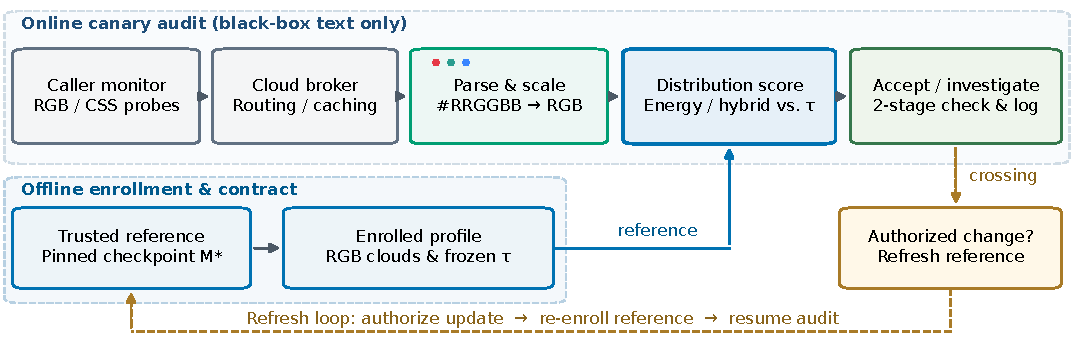
\includegraphics[width=\textwidth]{fig1_service_audit.pdf}
\caption{Consumer-side audit lifecycle for a brokered LLM service. Enrollment and protocol-matched probes feed a frozen consistency decision; configuration changes require investigation and reference refresh.}\label{fig:1}
\end{figure*}

\section{Methodology and Perturbation Analysis}

\subsection{Probes, Parsing, and RGB Coordinates}

The battery crosses 10 tasks with four languages (en, zh, ru, ar) for 40 task-language cells requesting random, favorite, warm, nature, ocean, calm, and night colors in hex (\texttt{\#RRGGBB}) and RGB syntax (Fig. 2; e.g., \emph{``Pick a random color. Reply with only its \#RRGGBB hex code.''}). Study S4 embeds color choices inside 1-line CSS custom properties (e.g., \texttt{-{}-brand-primary}) and 1-field JSON design tokens; Supplements C--F give complete inventories and verbatim prompts. After stripping reasoning fields and inline tags, the parser extracts the first valid \texttt{\#RRGGBB} code or validated $0\text{--}255$ RGB triplet and marks failures invalid. Valid parses retain canonical uppercase \texttt{\#RRGGBB}, coordinates, syntax, and a strict-only-color flag.


For an sRGB code $\mathbf c\in\Omega=\{0,\ldots,255\}^3$ \cite{ref24}, let $\mathbf x=T(\mathbf c)=100\mathbf c/255\in\Omega_{\mathrm{RGB}}=[0,100]^3$; clipped perturbations $\mathbf c'=\operatorname{clip}_{[0,255]^3}(\mathbf c+\boldsymbol\eta)$ with $\|\boldsymbol\eta\|_\infty\le a$ satisfy $\|T(\mathbf c')-T(\mathbf c)\|_2\le 100\sqrt3 a/255$. RGB100 linearly rescales channels without gamma inversion or Lab conversion and is used for all continuous scores; hard and soft voxels use raw channel units. Supplement A analyzes injective and Lipschitz color charts, and Supplement B ablates fixed-weight regularization.


\begin{figure*}[t]
\centering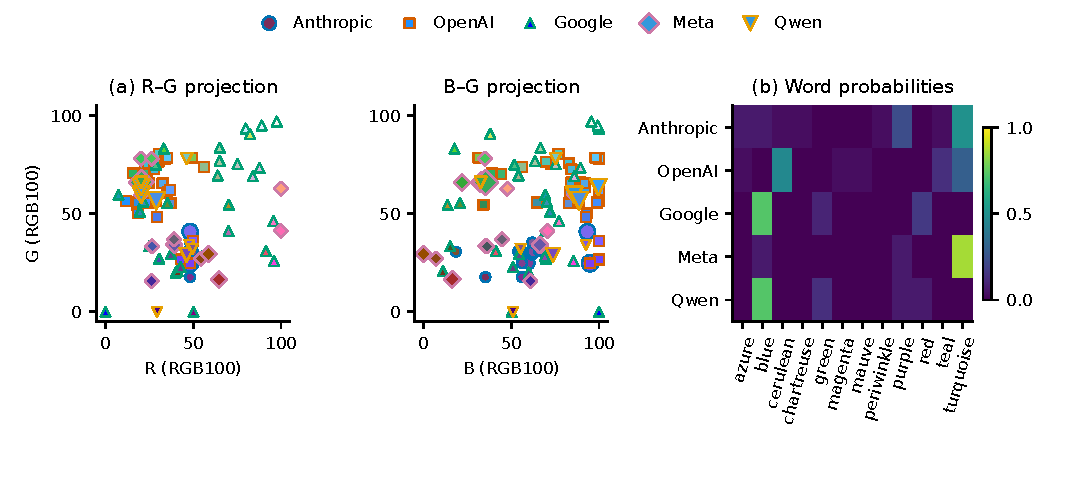
\includegraphics[width=\textwidth]{fig2_rgb_geometry_vs_words.pdf}
\caption{Five deterministically selected family representatives on the random-color probe. Marker area denotes output frequency and fill denotes actual RGB; the two projections show (R, G) and (B, G). Word probabilities use the matched endpoints and random-color word probe.}\label{fig:2}
\end{figure*}

\subsection{Discrete JSD and Support Escape}

With $M=(P+Q)/2$, base-2 JSD \cite{ref25} is


\begin{equation*}
\begin{aligned}D_{\mathrm{JSD}}(P\|Q)&=\tfrac12\sum_xP(x)\log_2\frac{P(x)}{M(x)}\\
&\quad+\tfrac12\sum_xQ(x)\log_2\frac{Q(x)}{M(x)},\end{aligned}
\end{equation*}

\noindent omitting zero-mass terms; it satisfies $0\le D_{\mathrm{JSD}}(P\|Q)\le 1$, equaling $1$ iff $\operatorname{supp}(P)\cap\operatorname{supp}(Q)=\emptyset$. $\Dhex{}$ uses exact RGB codes; $\Dvox{}$ uses $(\lfloor R/32\rfloor,\lfloor G/32\rfloor,\lfloor B/32\rfloor)$, giving $256^3$ and $8^3$ categories, respectively.


\begin{proposition}[Support-escape lower bound]\label{prop:1}\normalfont \emph{Fix a reference empirical distribution $P_{\mathrm{ref}}$ with support size $r$, and let $Q^{\mathrm{jitter}}$ draw source colors $\mathbf c\sim P_{\mathrm{src}}$ perturbed by independent uniform integer noise on $\{-a,\ldots,a\}^3$ ($a\ge1$) under the clipped transformation above. For $n$ i.i.d. draws $\hat Q_n^{\mathrm{jitter}}\sim Q^{\mathrm{jitter}}$ with support-escape probability $Q^{\mathrm{jitter}}(\Omega\setminus\operatorname{supp}(P_{\mathrm{ref}}))\ge t\in[0,1]$,}


\begin{equation*}
\mathbb E[\Dhex{}(P_{\mathrm{ref}},\hat Q_n^{\mathrm{jitter}})]\ge D_{\mathrm{JSD}}(P_{\mathrm{ref}}\|Q^{\mathrm{jitter}})\ge\psi(t),
\end{equation*}

\begin{equation}
\psi(t)=\tfrac12\log_2\frac2{2-t}+\tfrac{1-t}{2}\log_2\frac{2(1-t)}{2-t}+\tfrac t2\ge\tfrac t2,
\end{equation}

\noindent \emph{where $\psi$ is strictly increasing with $\psi(1)=1$ by continuity, and the population bound is tight. When $\operatorname{supp}(P_{\mathrm{src}})\subseteq\{a,\ldots,255-a\}^3$, one may take $t=\max(0,1-r/(2a+1)^3)$.}


\end{proposition}

Conditioning on observed query colors per cell and adding one random clipped shift per draw, Fig.~3(a) evaluates Eq.~(1) via the empirical query histogram's escape probability. Proposition~1 explains why genuine $D_{\mathrm{hex}}$ scores saturate toward $1$ under small channel shifts, while empirical EER depends jointly on the impostor distribution (Fig.~3(c)). Supplement~G proves Propositions~1--2 and Lemma~1.

\subsection{Soft Voxels and Regularized Energy}

With $w=48$ in original channel units and nodes $\mathcal I=\{0,\ldots,6\}^3$, define


\begin{equation}
\begin{aligned}W_i(\mathbf c)&=\prod_{d\in\{R,G,B\}}\max(0,1-|c_d/w-i_d|),\\
P_{\mathrm{soft}}(i\mid S)&=|S|^{-1}\sum_{\mathbf c\in S}W_i(\mathbf c).\end{aligned}
\end{equation}

Since $255/w=5.3125<6$, the trilinear tent weights satisfy $W_i(\mathbf c)\ge 0$ and $\sum_{i\in\mathcal I}W_i(\mathbf c)=1$ on $[0,255]^3$, so $P_{\mathrm{soft}}(\cdot\mid S)$ in Eq. (2) is a valid probability vector and $\Dsvox{}$ is the JSD between two soft histograms.


\begin{lemma}[Soft-voxel stability]\label{lem:1}\normalfont \emph{For $\mathbf c,\mathbf c'\in[0,255]^3$, $\|W(\mathbf c)-W(\mathbf c')\|_1\le(2/w)\|\mathbf c-\mathbf c'\|_1\le(6/w)\|\mathbf c-\mathbf c'\|_\infty$, so paired samples $S,S'$ shifted by at most $a$ per channel satisfy $D_{\mathrm{JSD}}(P_{\mathrm{soft}}(S)\|P_{\mathrm{soft}}(S'))\le b$ with $b=\min(1,3a/w)$.}


\end{lemma}

Fig. 3(b) plots this query-to-perturbed-query term $D_{\mathrm{JSD}}(P_{\mathrm{soft}}(S)\|P_{\mathrm{soft}}(S'))$. Against a fixed reference $P_{\mathrm{ref}}$, metric triangle inequality on $\sqrt{D_{\mathrm{JSD}}}$ gives $|\Delta\sqrt{\Dsvox{}}|\le\sqrt b$ and raw-score shift $|\Delta \Dsvox{}|\le\min(1,2\sqrt b)$; decision flips also depend on the score's margin to $\tau$.


For nonempty RGB100 clouds $U,V$, let $n=|U|$, $m=|V|$ and


\begin{equation*}
d_{UV}=\frac{\sum_{i,j}\|u_i-v_j\|_2}{nm},\qquad d_{UU}=\frac{\sum_{i,i'}\|u_i-u_{i'}\|_2}{n^2},
\end{equation*}

\noindent with $d_{VV}$ defined analogously, including diagonals. The V-statistic squared energy is $\widehat{\mathcal E}_V^2=2d_{UV}-d_{UU}-d_{VV}$. For distributions on $\mathbb R^3$ with finite first moments, population squared energy satisfies $\mathcal E^2(\mu,\nu)\ge 0$ with equality iff $\mu=\nu$ \cite{ref26,ref27}; applied to empirical measures, $0\le\widehat{\mathcal E}_V^2\le 2d_{UV}$. We therefore define


\begin{equation}
\Denergy{}=\frac{\widehat{\mathcal E}_V^2}{2d_{UV}},\qquad\Dereg{}=\frac{\widehat{\mathcal E}_V^2}{2d_{UV}+2\delta_0},
\end{equation}

\noindent where $\delta_0=15$ RGB100 length units in Eq. (3) and $\Denergy{}=0$ at $d_{UV}=0$. Floating-point evaluation clips $[\widehat{\mathcal E}_V^2]_+=\max(0,\widehat{\mathcal E}_V^2)$ to $[0,2d_{UV}]$ and sets scores to zero when $d_{UV}<10^{-12}$. For constant clouds separated by $\epsilon>0$ ($d_{UU}=d_{VV}=0, d_{UV}=\epsilon$), $\Denergy{}$ jumps from $0$ at $\epsilon=0$ to $1$; by contrast, $\Dereg{}=\epsilon/(\epsilon+\delta_0)\le\epsilon/\delta_0$ varies smoothly.


\begin{proposition}[Lipschitz stability of regularized energy ratios]\label{prop:2}\normalfont \emph{For nonempty $U,V\subset\mathbb R^3$, $\delta_0>0$, $d=d_{UV}$, and within-cloud mean distance average $h$ computed with diagonals ($\Dereg{}$) or without diagonals ($|U|,|V|\ge 2$, Section 3.7), let $F(d,h)=(d-h)/(d+\delta_0)$. Moving each point of $V$ by at most $\epsilon$ in Euclidean norm (in arbitrary directions) changes $F(d,h)$ and $[F(d,h)]_+$ by at most $2\epsilon/\delta_0$; moving every point of $U$ and $V$ by at most $\epsilon$ changes them by at most $4\epsilon/\delta_0$.}


\end{proposition}

For clipped ratios in $[0,1)$, channel shift $a$ bounds one-sided change by $\min\{1, 200\sqrt{3}a/(255\delta_0)\}$ ($0.0906$ at $a=1$, $0.7245$ at $a=8$ for $\delta_0=15$) and remains continuous as $d_{UV}\to 0$. Proposition~2 permits arbitrary worst-case per-point directions, but uncoordinated uniform jitter in Fig.~3(b) stays far below this envelope.

The Gaussian Bures--Wasserstein control \cite{ref28} fits biased covariances with ridge $10^{-3}I$ in squared RGB100 units and uses $\DWtwo{}=1-e^{-W_2/50}$ with a 50-unit RGB100 length scale. Unlike energy, matching two moments cannot distinguish all distributions; Supplement G gives its formula and limitations.


\begin{figure*}[t]
\centering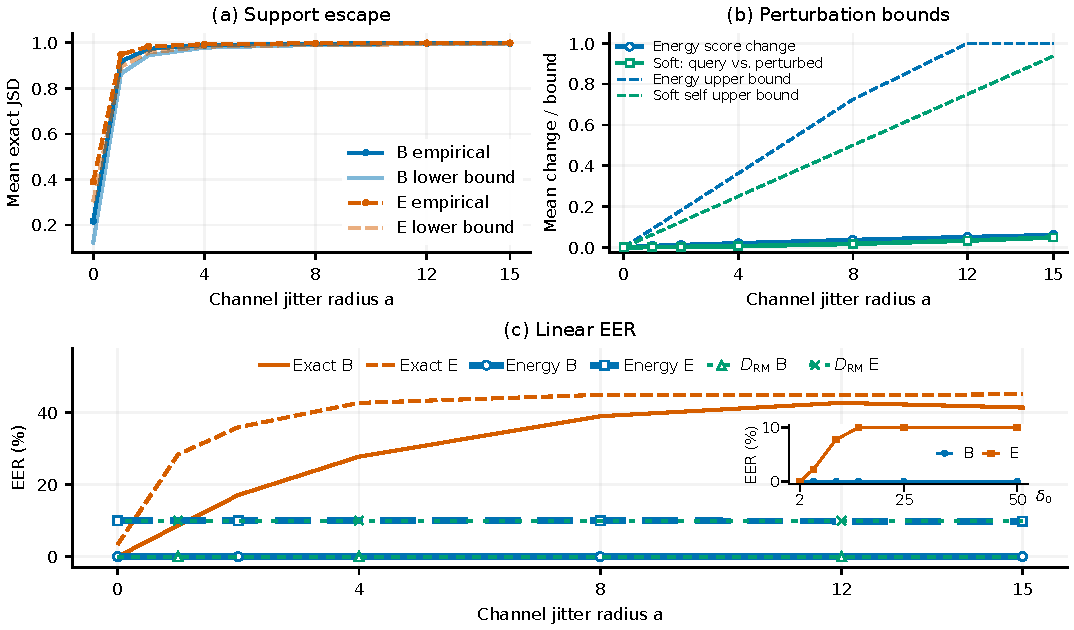
\includegraphics[width=\textwidth]{fig3_stability_bounds.pdf}
\caption{Ten fixed jitter seeds per radius. (a) Exact JSD and its clipping-aware conditional expected lower bound. (b) Energy score change and query-to-perturbed-query soft JSD with their respective upper bounds. (c) Re-swept linear EER; inset shows energy regularization sensitivity.}\label{fig:3}
\end{figure*}

\subsection{Composite Scores and Decisions}

$\Dside{}$ averages JSD over syntax (case/prefix or comma spacing), available first reasoning words, and log-binned reasoning lengths. Hex case tags distinguish all-digit codes (\texttt{numeric\_\allowbreak{}only}, $5.96\%$ of RGB), and reasoning lengths read API \texttt{usage.\allowbreak{}reasoning\_\allowbreak{}tokens} before falling back to visible character counts. $\Dside{}$ is thus an auxiliary syntax/envelope channel, not a color- or envelope-free invariant (Supplement B). Fixed composites, including the regularized multi-scale composite $\Drm{}$, are


\begin{equation}
\begin{aligned}\Dhyb{}&=0.35\Dvox{}+0.25\Dhex{}\\&\quad+0.25\Denergy{}+0.15\Dside{},\\\Dhybreg{}&=0.35\Dvox{}+0.25\Dhex{}\\&\quad+0.25\Dereg{}+0.15\Dside{},\\\Drm{}&=0.50\Dsvox{}+0.50\Dereg{}.\end{aligned}
\end{equation}

In Eq. (4), scores average shared eligible cells and accept at $S\le\tau$. Development genuine/impostor scores $G,I$ define $\tau_{\mathrm{mid}}=(\max G+\min I)/2$ and $\tau_{\mathrm{u0}}=\operatorname{nextafter}(\min I,-\infty)$ (zero FAR is guaranteed only on development negatives). AUC gives ties half weight, linear EER interpolates adjacent ROC points under re-swept thresholds, and frozen FAR/FRR evaluate deployment cutoffs.


\subsection{Enrollment Calibration and Equality Testing}

For each reference and cell, we bootstrap two enrollment-only clouds matching reference and planned query sizes across 256 fixed-seed draws, average across eligible cells to obtain $\mu_{\mathrm{self}}$ (using zero query data or test labels), and set $\Delta_D=D-\alpha\mu_{\mathrm{self}}$. Under IID enrollment sampling of size $n$, resampling $\hat P_n$ collides with probability $1/n$, scaling expected empirical within-sample distance (and the null bootstrap's unnormalized V-numerator) by $(n-1)/n$. Normalized $\Dereg{}$ ratios ($\overline{\mu}_{\mathrm{self}}/\overline{G}=0.732$ on B3v3, $0.598$ on E) reflect ratio normalization, not $(n-1)/n$. We compare raw scores, $\alpha=1$, and B-only leave-one-model-out selection over $\{0,0.25,0.5,1,1.5,2\}$ (breaking zero-error ties on B6v6/B8v7 toward $\alpha=1$). Protocol-specific B splits fit frozen thresholds: B3v3 (odd/\allowbreak{}even of six draws, 20 cells; used on E), B6v6 (first vs. next six draws, 20 cells; matched S1 check), and B8v7 (15 draws, 40 cells; min-5 valid per half for verification, min-1 for service-change calibration).


Adapting the two-sample energy test \cite{ref27} to stratified cells, we average $nm\widehat{\mathcal E}_V^2/(n+m)$ across cells over 999 within-cell label permutations with $p=(1+\#\{T_b\ge T_{\mathrm{obs}}\})/1000$. Rejection at $p\le0.05$ tests equal conditional valid-color distributions (pairwise rates are unadjusted and correlated across shared endpoints).


\subsection{Completion Baselines and Matched Budgets}

Adapting Gao et al.'s one-hot MMD and $L_1$ tests \cite{ref4} to raw strings (preserving whitespace, case, and invalid outputs, with empirical TV equal to $\tfrac12 L_1$), we evaluate $n,m\ge2$ with $k(s,t)=\mathbf1[s=t]$ via


\begin{equation*}
\begin{aligned}\widehat{\mathrm{MMD}}_u^2&=\frac{\sum_{i\ne i'}k(x_i,x_{i'})}{n(n-1)}+\frac{\sum_{j\ne j'}k(y_j,y_{j'})}{m(m-1)}\\
&\quad-\frac{2\sum_{i,j}k(x_i,y_j)}{nm},\end{aligned}
\end{equation*}

\noindent averaging per-cell statistics (exact rational MMD-U) over 999 permutations and reporting statistic EER/AUC separately from rejection rates. Invalid parses still consume call budgets. S3 tests $N\in\{6,10,20,30\}$ ($n=m=N/2$) across up to 40 shared $K$-cell subsets ($K=1,\ldots,10$; B-20\ensuremath{\times}6/D test $N=6$), and ten fixed seeds perturb parsed RGB literals in memory.


\subsection{Finite-Sample Energy Estimators}

For independent IID samples of sizes $n,m$ ($a_P=\mathbb E\|X-X'\|$, $a_Q=\mathbb E\|Y-Y'\|$), the nonnegative V numerator satisfies $\mathbb E[\widehat{\mathcal E}_V^2]=\mathcal E^2(P,Q)+a_P/n+a_Q/m$. For $n,m\ge2$, the U numerator


\begin{equation*}
\widehat{\mathcal E}_U^2=2d_{UV}-\frac{n}{n-1}d_{UU}-\frac{m}{m-1}d_{VV}
\end{equation*}

\noindent lies in $[-2d_{UV},2d_{UV}]$, may be negative, and is unbiased for $\mathcal E^2(P,Q)$ under independent IID sampling. Table 7 compares $\Dereg{}$ (\emph{V regularized}) and centered $\Dereg{}$ (\emph{V self-centered}) against three U-statistic forms: $\widehat{\mathcal E}_U^2$ (\emph{U numerator}), $\widehat{\mathcal E}_U^2/(2d_{UV}+2\delta_0)$ (\emph{U signed ratio}), and $[\widehat{\mathcal E}_U^2]_+/(2d_{UV}+2\delta_0)$ (\emph{U clipped ratio}, strictly in $[0,1)$ since $\delta_0>0$, so $\min\{1,\cdot\}$ is inactive). Neither random-denominator normalization nor clipping preserves unbiasedness; Proposition 2 gives both U ratios $2\epsilon/\delta_0$ one-sided and $4\epsilon/\delta_0$ two-sided bounds.


All U-statistic variants and matched V-statistic controls are evaluated over identical cells containing at least two valid responses per side.

\section{Experimental Design and Dataset Architecture}

\subsection{Datasets and Reproducibility Architecture}

Five baseline datasets (A--E, Oct. 2026; 11,888 unique calls) and four online studies (S1--S4, Nov. 2026; 22,640 calls) provide \textbf{34,528} unique cloud responses (Table 1), backed by read-only JSONL logs, deduplication rules, SHA-256 input manifests, fixed seeds, and offline analysis/plotting scripts.


\begin{table*}[t]
\centering
\caption{Cloud Response Datasets}
\label{tab:source-1}
\footnotesize
\setlength{\tabcolsep}{3pt}
\renewcommand{\arraystretch}{1.08}
\begin{tabular}{@{}>{\raggedright\arraybackslash}p{\dimexpr 0.209877\textwidth-6pt\relax}>{\raggedright\arraybackslash}p{\dimexpr 0.135802\textwidth-6pt\relax}>{\raggedright\arraybackslash}p{\dimexpr 0.197531\textwidth-6pt\relax}>{\raggedright\arraybackslash}p{\dimexpr 0.074074\textwidth-6pt\relax}>{\raggedright\arraybackslash}p{\dimexpr 0.123457\textwidth-6pt\relax}>{\raggedright\arraybackslash}p{\dimexpr 0.259259\textwidth-6pt\relax}@{}}
\toprule
Suite /\allowbreak{} Dataset & Models /\allowbreak{} Endpoints & Probe Grid (Cells $\times$ Reps) & Unique Calls & Valid Parsed (Rate) & Primary Evaluation Objective \\
\midrule
\textbf{Dataset A} (Census) & 56 (11 families) & $8 \times 6$ (4 tasks $\times$ \texttt{en/\allowbreak{}zh}) & 2,688 & 2,611 (97.14\%) & Broad census, family/sublineage EER, side-channel check \\
\textbf{Dataset B} (Dev Scaling) & 10 dev models & $40 \times 15$ (10 tasks $\times$ 4 langs) & 5,520 & 5,932/6,000 (98.87\%) & $(n,k)$ budget grid, service-change tests, threshold calibration \\
\textbf{Dataset C} (Paraphrase) & 10 dev models & $16 \times 8$ ($P_1, P_2$ rewordings) & 1,280 & 1,262 (98.59\%) & Within-pool verification vs. $P_0 \to P_1/P_2$ template shift \\
\textbf{Dataset D} (Word Baseline) & 10 dev models & $20 \times 6$ (10 word tasks $\times$ \texttt{en/\allowbreak{}zh}) & 1,200 & 1,196 (99.67\%) & Call-parity word baseline vs. \texttt{B-\allowbreak{}20x6} \\
\textbf{Dataset E} (Held-Out) & 10 non-B models & $20 \times 6$ (10 color tasks $\times$ \texttt{en/\allowbreak{}zh}) & 1,200 & 1,187 (98.92\%) & \texttt{+6.\allowbreak{}74h} \texttt{A-\allowbreak{}>E} check, frozen \texttt{B-\allowbreak{}>E} transfer, OOS jitter \\
\textbf{Study S1} (\texttt{T+21.\allowbreak{}3d} \& GW) & 14 $\times$ 2 gateways & $20 \times 6$ (\texttt{CF} \& \texttt{OR} gateways) & 3,360 & 3,338 (99.35\%) & 21.32-day drift \& \texttt{CF <-\allowbreak{}> OR} cross-gateway transfer \\
\textbf{Study S2} (Multi-Provider) & 6 weights $\times$ 3 hosts & $20 \times 6$ (12 pinned backends) & 2,160 & 2,147 (99.40\%) & Cross-host matching (\texttt{int4}/\texttt{fp4}/\texttt{fp8}/\texttt{bf16}/LPU) \\
\textbf{Study S3} (Locked Parity) & 20 (8 families) & $10 \times 30 \times 2$ (completion cap 64) & 12,000 & 11,985 (99.88\%) & Matched 15v15 parity benchmark against Bruckner with a 64-token cap \\
\textbf{Study S4} (Structured Canaries) & 20 (8 families) & \texttt{S4a} $16\times 10$ + \texttt{S4b} $16\times 6$ & 5,120 & 5,087 (99.36\%) & CSS/JSON canary parsing and gateway regex pass rates \\
\bottomrule
\end{tabular}
\par\vspace{3pt}\begin{minipage}{\textwidth}\footnotesize B: 5,520 unique calls + 480 A rows (6,000). Three of 12,000 S3 responses reached the length limit (two color, one word; one valid).\end{minipage}
\end{table*}

\subsection{Decoding Hyperparameters and Temperature Handling Across Modern APIs}

Requests disable optional thinking where supported and set completion caps of 16--256 tokens (locked at 64 in S2/S3 and 128 in S4; Supplement K). Datasets A--C omit explicit temperature (\texttt{temperature\_\allowbreak{}sent=\allowbreak{}null}). D, E, and \texttt{S1\_\allowbreak{}CF21} pass \texttt{temperature=\allowbreak{}1.\allowbreak{}0} only on direct Workers AI calls (1--2 endpoints), while \texttt{S1\_\allowbreak{}OR21}, S2, S3, and S4 send \texttt{temperature=\allowbreak{}1.\allowbreak{}0} uniformly (with recorded stripping shared across paired requests on two S3 Claude endpoints). In S1, \texttt{OR21} sets \texttt{reasoning.\allowbreak{}effort=\allowbreak{}"low"} on five reasoning endpoints, and Cloudflare maps \texttt{llama-\allowbreak{}3.\allowbreak{}3-\allowbreak{}70b-\allowbreak{}fp8-\allowbreak{}fast} to a speculative-decoding (\texttt{-\allowbreak{}sd}) variant absent on OpenRouter. S2 disables provider fallbacks (\texttt{0/\allowbreak{}18} mixed), but OpenRouter load-balances 5/14 \texttt{S1\_\allowbreak{}OR21}, 7/20 S3, and 5--6/20 S4 endpoints across sub-providers (S3 odd/\allowbreak{}even sub-provider TV mean 0.0419, max 0.1200). In A, 144 records expose reasoning summaries without raw text. In S3, sub-provider \texttt{GMICloud} (\texttt{s3-\allowbreak{}deepseek-\allowbreak{}v3.\allowbreak{}2}, 158/300 calls) ignored thinking suppression and billed up to 907 output tokens; parsing strips reasoning traces while overhead accounting retains all billed tokens.


\section{Empirical Evaluation: Baseline and Live External-Validity Studies}

\subsection{56-Endpoint Census and Formatting Side-Channel Ablation (Dataset A)}

On Dataset A (56 endpoints across 11 families, 8 cells $\times$ 6 repetitions, 3v3 split with $\ge 2$ valid responses per half), we evaluate 56 genuine pairs against 3,080 all-pairs, 2,958 cross-sublineage, and 2,476 cross-vendor-family impostors, plus leave-one-out 1-NN family attribution over 50 multi-member-family models (Table 2).


\begin{table*}[t]
\centering
\caption{Dataset A (56 Models, $8\times 6$ Shallow Budget) Verification and Family Attribution}
\label{tab:source-2}
\footnotesize
\setlength{\tabcolsep}{3pt}
\renewcommand{\arraystretch}{1.08}
\begin{tabular}{@{}>{\raggedright\arraybackslash}p{\dimexpr 0.073394\textwidth-6pt\relax}>{\raggedright\arraybackslash}p{\dimexpr 0.073394\textwidth-6pt\relax}>{\raggedright\arraybackslash}p{\dimexpr 0.192661\textwidth-6pt\relax}>{\raggedright\arraybackslash}p{\dimexpr 0.247706\textwidth-6pt\relax}>{\raggedright\arraybackslash}p{\dimexpr 0.211009\textwidth-6pt\relax}>{\raggedright\arraybackslash}p{\dimexpr 0.201835\textwidth-6pt\relax}@{}}
\toprule
Metric & AUC & Discrete /\allowbreak{} linear EER & Cross-sublineage linear EER & Cross-family linear EER & LOO family attribution \\
\midrule
$\Denergy{}$ & 0.9900 & 5.06\% /\allowbreak{} 4.77\% & 3.75\% & 3.57\% & 31/50 (62.00\%) \\
$\Dereg{}$ & 0.9872 & 5.36\% /\allowbreak{} 5.36\% & 5.36\% & 4.52\% & 35/50 (70.00\%) \\
$\Dhyb{}$ & 0.9774 & 7.14\% /\allowbreak{} 7.14\% & 7.14\% & 7.14\% & 36/50 (72.00\%) \\
$\Dhex{}$ & 0.9588 & 10.73\% /\allowbreak{} 10.71\% & 10.71\% & 8.93\% & 38/50 (76.00\%) \\
$\Drm{}$ & 0.9582 & 8.93\% /\allowbreak{} 8.93\% & 8.93\% & 8.93\% & 34/50 (68.00\%) \\
$\Dvox{}$ & 0.9489 & 8.83\% /\allowbreak{} 8.93\% & 8.93\% & 8.93\% & 39/50 (78.00\%) \\
$\Dside{}$ & 0.7804 & 30.32\% /\allowbreak{} 30.32\% & 29.76\% & 28.56\% & 17/50 (34.00\%) \\
\bottomrule
\end{tabular}
\par\vspace{3pt}\begin{minipage}{\textwidth}\footnotesize Archived \texttt{evaluate\_\allowbreak{}cohort}/\texttt{within} requires $\ge 2$ valid parses in both halves per endpoint before pairing; side-independent filtering ($\ge 2$ enrollment parses for $i$, $\ge 2$ query parses for $j$, intersected) alters 163/3,080 negatives (0/56 genuine), giving 4.16\% vs. 4.77\% linear EER for $\Denergy{}$ and unchanged 5.36\% for $\Dereg{}$ (\texttt{scripts/\allowbreak{}sensitivity\_\allowbreak{}checks.\allowbreak{}py}).\end{minipage}
\end{table*}

Continuous distances lead binary verification in Table 2, while family attribution favors categorical retention (39/50 under $\Dvox{}$ vs. 35/50 under $\Dereg{}$). Merging \texttt{numeric\_\allowbreak{}only} hex tags into \texttt{upper} and stripping API reasoning telemetry lowers $\Dside{}$ AUC/EER from 0.7804/30.32\% to 0.6557/36.76\% on A and from 0.9722/10.00\% to 0.6933/36.00\% on B (Supplement B). Relaxing valid-cell eligibility from $\ge 2$ to $\ge 1$ for thinking-truncated \texttt{gw-\allowbreak{}gemini-\allowbreak{}2.\allowbreak{}5-\allowbreak{}flash} gives 5.62\% $\Denergy{}$ and unchanged 5.36\% $\Dereg{}$ EER.


\subsection[Query-Budget Scaling and (n, k) Grid Ablation (Dataset B)]{\boldmath Query-Budget Scaling and $(n, k)$ Grid Ablation (Dataset B)}

Increasing B to 40 cells and 15 repetitions yields AUC 1.0000 and 0.00\% discrete and linear EER for all six nonparametric color metrics. Gaussian $\DWtwo{}$ retains 2.22\% linear EER (1.11\% discrete, 0.9978 AUC) due to the two-moment limit in Section 3.3. In Fig. 4(a), coverage and depth interact: 60 draws at $(n=15,k=4)$ give 1.78\% mean linear EER, while 96 draws at $(n=6,k=16)$ give 0.46\%.


\begin{figure*}[t]
\centering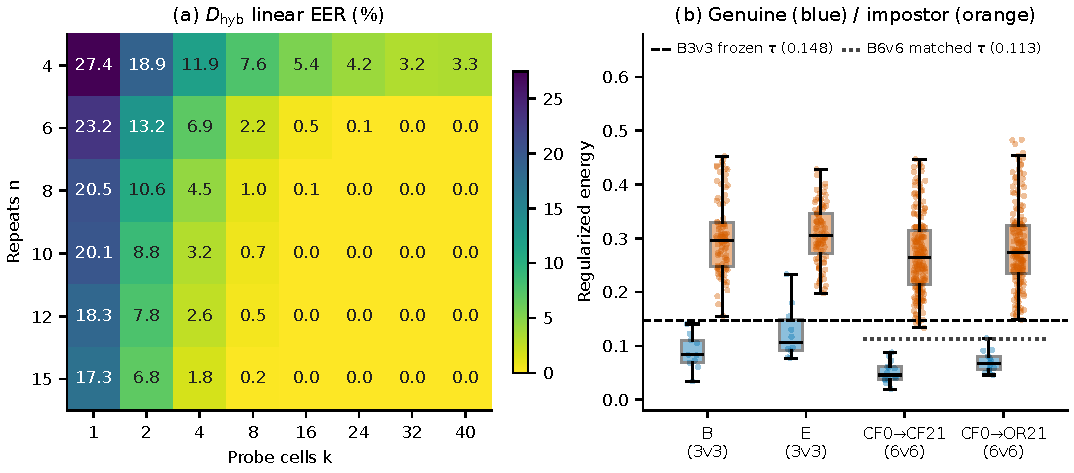
\includegraphics[width=\textwidth]{fig4_budget_and_drift.pdf}
\caption{(a) Mean $\Dhyb{}$ linear EER over the B sampling-budget grid. (b) Genuine and impostor regularized-energy scores across B ($20\times 6$, 3v3), E ($20\times 6$, 3v3), and S1 paths ($20\times 6$, 6v6), with frozen B3v3 ($\tau=0.148$, dashed) and budget-matched B6v6 ($\tau=0.113$, dotted) midpoint thresholds.}\label{fig:4}
\end{figure*}

\subsection{Within-Pool Self-Verification vs.\ Cross-Template Shift (Dataset C)}
Dataset C evaluates two paraphrase pools across eight bilingual cells (eight repetitions per cell): syntactic rewording $P_1$ and design-contextual framing $P_2$ (detailed per-metric results in Supplement~I). Regularized energy $\Dereg{}$ achieves 0.00\% and 1.11\% linear EER within $P_1$ and $P_2$, respectively. Cross-template comparisons $P_0 \rightarrow P_1$ and $P_0 \rightarrow P_2$ yield 17.78\% and 11.11\% EER. Because even synonymous phrasing shifts conditional color priors, reference profiles must remain conditioned on the exact prompt battery.

\subsection{Matched Probe and Statistic Comparisons (Dataset D and Study S3)}

\textbf{Structured color elicitation.} Averaging 40 overlapping 10-cell subsets ($K=10$, three draws/cell/side, 30 calls/side) across the 10 development models on B-20\ensuremath{\times}6 and D yields clean EERs of 0.94\% (Color MMD-U) and 1.00\% ($\Dereg{}$) vs. 4.52\% (Word MMD-U) and 5.23\% (Word JSD). At $K=20$ (60 calls/side), all metrics except Word JSD (1.11\% Word JSD; Supplement K) reach 0.00\% EER. Color vs. word probes yield 18.65 vs. 7.05 distinct valid outputs/cell (111,305 vs. 79,398 tokens); at $K=10$ under $\pm8$ jitter, B-20\ensuremath{\times}6 EER is 49.73\% (Color MMD-U) vs. 1.59\% ($\Dereg{}$). Because D also queries animals, cities, numbers, letters, and coins, full-battery gaps reflect joint prompt-and-coordinate efficiency. S3 tests 20 models (8 families, 10 English probes, 15v15, cap 64; Table 3), parsing 99.97\% color (5,998/6,000) and 99.78\% word (5,987/6,000) calls. On S3's two shared color-concept tasks under raw-string MMD-U (\texttt{hex\_\allowbreak{}random}, \texttt{hex\_\allowbreak{}favorite} vs. \texttt{brk\_\allowbreak{}rand\_\allowbreak{}color}, \texttt{brk\_\allowbreak{}fav\_\allowbreak{}color}; Supplement K), hex coordinates raise 3v3/15v15 AUC from 0.8349/0.9784 to 0.9156/0.9909 (17.92\% vs. 20.21\% and 5.26\% vs. 5.00\% EER) and enable 3D continuous distances.


\begin{table*}[t]
\centering
\caption{S3 Matched-Budget Raw-Statistic Linear EER; Final Column Averages Ten RGB Jitter Seeds}
\label{tab:source-3}
\footnotesize
\setlength{\tabcolsep}{3pt}
\renewcommand{\arraystretch}{1.08}
\begin{tabular}{@{}>{\raggedright\arraybackslash}p{\dimexpr 0.098765\textwidth-6pt\relax}>{\raggedright\arraybackslash}p{\dimexpr 0.209877\textwidth-6pt\relax}>{\raggedright\arraybackslash}p{\dimexpr 0.098765\textwidth-6pt\relax}>{\raggedright\arraybackslash}p{\dimexpr 0.098765\textwidth-6pt\relax}>{\raggedright\arraybackslash}p{\dimexpr 0.098765\textwidth-6pt\relax}>{\raggedright\arraybackslash}p{\dimexpr 0.098765\textwidth-6pt\relax}>{\raggedright\arraybackslash}p{\dimexpr 0.098765\textwidth-6pt\relax}>{\raggedright\arraybackslash}p{\dimexpr 0.098765\textwidth-6pt\relax}>{\raggedright\arraybackslash}p{\dimexpr 0.098765\textwidth-6pt\relax}@{}}
\toprule
N & Probe /\allowbreak{} statistic & K=1 & K=2 & K=4 & K=6 & K=8 & K=10 & K=10, \ensuremath{\pm}8 \\
\midrule
6 & Color MMD-U & 25.32\% & 16.99\% & 10.03\% & 6.58\% & 4.95\% & 3.49\% & 50.01\% \\
6 & Color $\Dereg{}$ & 25.00\% & 17.84\% & 12.09\% & 8.99\% & 6.10\% & 5.00\% & 5.00\% \\
6 & Color $\Dhex{}$ & 25.89\% & 19.96\% & 16.92\% & 13.33\% & 11.06\% & 10.00\% & 41.21\% \\
6 & Word MMD-U & 32.14\% & 22.81\% & 14.87\% & 10.99\% & 8.34\% & 8.04\% & --- \\
6 & Word JSD & 33.17\% & 24.81\% & 17.54\% & 15.37\% & 10.96\% & 6.25\% & --- \\
10 & Color MMD-U & 18.43\% & 10.96\% & 5.34\% & 2.43\% & 1.12\% & 0.00\% & 49.93\% \\
10 & Color $\Dereg{}$ & 19.56\% & 11.05\% & 5.47\% & 2.64\% & 0.79\% & 0.26\% & 0.50\% \\
20 & Color MMD-U & 13.52\% & 5.54\% & 2.61\% & 1.06\% & 0.43\% & 0.26\% & 50.02\% \\
20 & Color $\Dereg{}$ & 14.99\% & 5.54\% & 3.30\% & 0.77\% & 0.08\% & 0.00\% & 0.53\% \\
30 & Color MMD-U & 12.50\% & 4.60\% & 1.15\% & 0.25\% & 0.09\% & 0.00\% & 50.00\% \\
30 & Color $\Dereg{}$ & 13.56\% & 4.95\% & 1.32\% & 0.26\% & 0.07\% & 0.00\% & 0.00\% \\
30 & Color $\Dhex{}$ & 15.27\% & 10.05\% & 7.59\% & 5.16\% & 4.84\% & 5.00\% & 35.40\% \\
30 & Color TV & 14.19\% & 10.06\% & 8.07\% & 5.21\% & 4.74\% & 5.00\% & 35.99\% \\
30 & Word MMD-U & 19.23\% & 8.77\% & 4.31\% & 3.36\% & 1.90\% & 1.32\% & --- \\
30 & Word JSD & 22.99\% & 12.52\% & 7.76\% & 6.06\% & 5.04\% & 5.00\% & --- \\
\bottomrule
\end{tabular}
\end{table*}

\textbf{Continuous RGB comparison.} On S3 ($K=10$), $N=6$ yields 3.49\% (Color MMD-U) and 5.00\% ($\Dereg{}$) vs. 8.04\% (Word MMD-U), 6.25\% (Word JSD), and 10.00\% empirical $\Dhex{}$. Canonical \texttt{\#RRGGBB} vs. normalized-word MMD-U keeps this gain (5.00\% vs. 9.31\% at $N=6$; 0.00\% vs. 0.53\% at $N=30$). At $N=30$, Color MMD-U and $\Dereg{}$ reach 0.00\% clean EER (1.0000 AUC) vs. 1.32\% (Word MMD-U) and 5.00\% ($\Dhex{}$, Color TV, Word JSD). Under controlled $\pm8$ jitter, Color MMD-U, TV, and $\Dhex{}$ degrade to 50.00\% (0.5184 AUC), 35.99\%, and 35.40\% EER, while $\Dereg{}$ holds 0.00\% (Fig. 5). At $p\le0.05$, Color MMD-U rejects 10.00\% genuine and 100.00\% impostor pairs cleanly, rising to 100.00\% under jitter (Sections 3.5--3.6).


\begin{figure*}[t]
\centering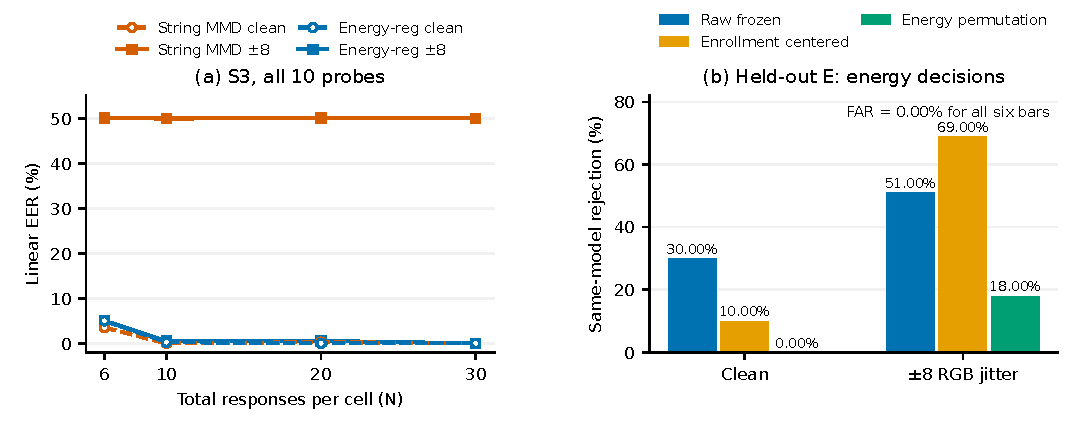
\includegraphics[width=\textwidth]{fig5_geometry_and_calibration.pdf}
\caption{(a) S3 EER for string MMD and regularized energy on the same color responses across budgets. (b) Held-out E same-model rejection: raw and centered frozen rules, and per-audit energy permutation testing at $p\le0.05$. FAR is zero throughout; jitter results average ten fixed seeds.}\label{fig:5}
\end{figure*}

\textbf{RGB output modes.} In S3, exact CSS named colors account for 14.25\% of unanchored, 49.29\% of semantic, and 64.89\% of preference responses, while repeated-nibble codes constitute 23.85\% of preference responses. Familiar color literals and structured encoding habits thus form distinct behavioral modes shaped by pre-training exposure to frontend code and stylesheets (Fig.~2) and concentrate mass onto model-specific regions of $\Omega_{\mathrm{RGB}}$.

\subsection{Held-Out, Longitudinal, and Gateway Transfer (Dataset E and Study S1)}
\textbf{Held-out transfer.} Dataset E comprises 10 models absent from B, collected a median 6.74~h after A. Transferring frozen B3v3 cutoffs yields E FRR/FAR of 10.00\%/0.00\% for $\Dhyb{}$ ($\tau = 0.348407$) and 30.00\%/0.00\% for raw $\Dereg{}$ ($\tau = 0.148017$, re-swept EER 10.00\%).

\textbf{Longitudinal and cross-gateway audit (S1).} Across two observations $21.07\text{--}21.32$~d apart (median 21.32~d), we re-audited 14 provider-declared endpoints on Cloudflare AI Gateway (CF) and OpenRouter (OR) over 20 bilingual cells $\times$ 6 draws (3,360 calls; 99.23\% and 99.46\% valid). This cohort pairs B's 10 development models (\texttt{CF0} shares 1,200 enrollment rows with B calibration) with four held-out E models (\texttt{heldout4}, disjoint from B; Section~5.7). Table~4 evaluates 6v6 scores under frozen B3v3. Budget-matched B6v6 appears in Table~5, where raw $\mathrm{CF0}\rightarrow\mathrm{OR21}$ rejects \texttt{cf-qwen2.5-coder-32b} (1/4 = 25.00\% raw \texttt{heldout4} FRR vs.\ 0.00\% centered). Against all 13 non-self models ($4\times 13 = 52$ open-set impostors vs.\ 12 within-slice), raw B3v3 yields 1/52 (1.92\%) FAR on $\mathrm{CF0}\rightarrow\mathrm{CF21}$ (\texttt{gw-gpt-4.1}$\rightarrow$\texttt{gw-gpt-4o}, score $0.1336$) and 0.00\% centered or under B6v6.

\begin{table*}[t]
\centering
\caption{Study S1 Longitudinal ($T+21.32\text{d}$) and Cloudflare $\leftrightarrow$ OpenRouter Cross-Gateway Verification (14 Genuine vs.\ 182 Impostors)}
\label{tab:s1_transfer}
\footnotesize\setlength{\tabcolsep}{3pt}\renewcommand{\arraystretch}{1.05}
\begin{tabular*}{\textwidth}{@{\extracolsep{\fill}}llccccc@{}}
\toprule
Enrollment $\rightarrow$ Query (6v6) & Metric & Top-1 & AUC & Linear EER & Genuine /\allowbreak{} Impostor Mean & Frozen B3v3 FRR /\allowbreak{} FAR \\
\midrule
$\mathrm{CF0} \rightarrow \mathrm{CF21}$ & $\Drm{}$ & 14/14 & 1.0000 & 0.00\% & 0.0728 /\allowbreak{} 0.3544 & 0.00\% /\allowbreak{} 1.10\% \\
$\mathrm{CF0} \rightarrow \mathrm{CF21}$ & $\Dereg{}$ & 14/14 & 1.0000 & 0.00\% & 0.0511 /\allowbreak{} 0.2690 & 0.00\% /\allowbreak{} 2.20\% \\
$\mathrm{CF0} \rightarrow \mathrm{CF21}$ & $\Dhyb{}$ & 14/14 & 1.0000 & 0.00\% & 0.1600 /\allowbreak{} 0.5348 & 0.00\% /\allowbreak{} 0.55\% \\
$\mathrm{CF0} \rightarrow \mathrm{CF21}$ (heldout4) & $\Dereg{}$ & 4/4 & 1.0000 & 0.00\% & 0.0599 /\allowbreak{} 0.2989 & 0.00\% /\allowbreak{} 0.00\% \\
$\mathrm{CF0} \rightarrow \mathrm{CF21}$ (heldout4) & $\Dhyb{}$ & 4/4 & 1.0000 & 0.00\% & 0.1790 /\allowbreak{} 0.5721 & 0.00\% /\allowbreak{} 0.00\% \\
$\mathrm{CF21} \rightarrow \mathrm{OR21}$ & $\Drm{}$ & 14/14 & 1.0000 & 0.00\% & 0.0864 /\allowbreak{} 0.3613 & 0.00\% /\allowbreak{} 0.00\% \\
$\mathrm{CF21} \rightarrow \mathrm{OR21}$ & $\Dereg{}$ & 14/14 & 1.0000 & 0.00\% & 0.0619 /\allowbreak{} 0.2809 & 0.00\% /\allowbreak{} 0.55\% \\
$\mathrm{CF21} \rightarrow \mathrm{OR21}$ & $\Dhyb{}$ & 14/14 & 1.0000 & 0.00\% & 0.1834 /\allowbreak{} 0.5543 & 0.00\% /\allowbreak{} 0.00\% \\
$\mathrm{CF0} \rightarrow \mathrm{OR21}$ & $\Drm{}$ & 14/14 & 1.0000 & 0.00\% & 0.0937 /\allowbreak{} 0.3642 & 0.00\% /\allowbreak{} 1.10\% \\
$\mathrm{CF0} \rightarrow \mathrm{OR21}$ & $\Dereg{}$ & 14/14 & 1.0000 & 0.00\% & 0.0697 /\allowbreak{} 0.2830 & 0.00\% /\allowbreak{} 0.00\% \\
$\mathrm{CF0} \rightarrow \mathrm{OR21}$ & $\Dhyb{}$ & 14/14 & 1.0000 & 0.00\% & 0.1960 /\allowbreak{} 0.5564 & 0.00\% /\allowbreak{} 0.00\% \\
\bottomrule
\end{tabular*}
\end{table*}

\textbf{Enrollment self-dispersion calibration.} Centering $\Delta_D=D-\alpha\mu_{\mathrm{self}}$ ($\alpha=1$) sets raw/centered cutoffs to 0.148017/0.073044 on B3v3 and 0.113100/0.060830 on B6v6. It cuts clean E FRR, longitudinal S1 FAR, and B8v7 50\%-routing false acceptance (31.11\% to 14.44\%, Supplement L). Because $D\le\tau_{\mathrm{self}}+\mu_{\mathrm{self}}(M^*)$ adds no query-noise slack, jittered E FRR rises (Table 5).


\begin{table}[t]
\centering
\caption{Frozen Regularized-Energy Transfer; Self Uses B-Selected $\alpha=1$}
\label{tab:source-5}
\footnotesize
\setlength{\tabcolsep}{3pt}
\renewcommand{\arraystretch}{1.08}
\begin{tabular}{@{}>{\raggedright\arraybackslash}p{\dimexpr 0.211538\columnwidth-6pt\relax}>{\raggedright\arraybackslash}p{\dimexpr 0.250000\columnwidth-6pt\relax}>{\raggedright\arraybackslash}p{\dimexpr 0.269231\columnwidth-6pt\relax}>{\raggedright\arraybackslash}p{\dimexpr 0.269231\columnwidth-6pt\relax}@{}}
\toprule
Condition & B calibration & Raw FRR /\allowbreak{} FAR & Self FRR /\allowbreak{} FAR \\
\midrule
E clean & B3v3 & 30.00\% /\allowbreak{} 0.00\% & 10.00\% /\allowbreak{} 0.00\% \\
E \ensuremath{\pm}8 & B3v3 & 51.00\% /\allowbreak{} 0.00\% & 69.00\% /\allowbreak{} 0.00\% \\
CF0 \ensuremath{\rightarrow} CF21 & B3v3 & 0.00\% /\allowbreak{} 2.20\% & 0.00\% /\allowbreak{} 0.00\% \\
CF21 \ensuremath{\rightarrow} OR21 & B3v3 & 0.00\% /\allowbreak{} 0.55\% & 0.00\% /\allowbreak{} 0.55\% \\
CF0 \ensuremath{\rightarrow} OR21 & B3v3 & 0.00\% /\allowbreak{} 0.00\% & 0.00\% /\allowbreak{} 0.00\% \\
CF0 \ensuremath{\rightarrow} CF21 & B6v6 & 0.00\% /\allowbreak{} 0.00\% & 0.00\% /\allowbreak{} 0.00\% \\
CF21 \ensuremath{\rightarrow} OR21 & B6v6 & 7.14\% /\allowbreak{} 0.00\% & 0.00\% /\allowbreak{} 0.55\% \\
CF0 \ensuremath{\rightarrow} OR21 & B6v6 & 7.14\% /\allowbreak{} 0.00\% & 0.00\% /\allowbreak{} 0.00\% \\
\bottomrule
\end{tabular}
\end{table}

\textbf{Ranking, frozen cutoffs, and equality testing under drift.} Stratified Sz\'{e}kely--Rizzo testing yields 0.00\% clean and 18.00\% jitter FRR on E at 0.00\% FAR (Fig. 5(b)). Across S1's CF0\ensuremath{\rightarrow}CF21, CF21\ensuremath{\rightarrow}OR21, and CF0\ensuremath{\rightarrow}OR21 paths, equality tests ($p\le0.05$) reject 7.14\%, 28.57\%, and 42.86\% of declared genuine pairs for energy and 7.14\%, 21.43\%, and 28.57\% for Color MMD-U (100\% of impostors; 22.22\% and 44.44\% for energy on the nine endpoints without \texttt{reasoning.\allowbreak{}effort} overrides, Supplement K). By contrast, $\Dereg{}$, $\Drm{}$, $\Dhyb{}$, and raw-string Color MMD-U keep 0.00\% EER across all 14 endpoints and subgroups with low frozen FAR/FRR (Tables 4--5). This complements the shallow-sample, cross-host, and perturbation gains of continuous and hybrid RGB metrics (Tables 2--3; Sections 5.4, 5.6, 6.1).


\subsection{Multi-Provider Serving Stacks and Precision Configurations (Study S2)}
Study S2 audits 18 endpoints covering six open-weight checkpoints across three providers each, spanning 12 pinned cloud backends (DeepInfra, Parasail, Cloudflare, Groq LPU, SiliconFlow, AtlasCloud, Mistral, Venice, DekaLLM, Crusoe, Fireworks, and CoreWeave) with fallback disabled across all 2,160 confirmed calls. Serving regimes include matched \texttt{fp8}, Fireworks \texttt{int4} vs.\ CoreWeave \texttt{bf16}, DeepInfra \texttt{fp4} vs.\ SiliconFlow \texttt{fp8}, and Groq LPU vs.\ GPU \texttt{fp8} (Supplement~J).

Treating same-checkpoint cross-provider pairs as positives and high-to-low-bit queries as anomalies (LPU/official unspecified), the four high-to-low-bit pairs vs. 20 high-precision controls yield 0.8250/30.00\% AUC/EER for $\Dhyb{}$ and 0.5250/50.00\% for $\Dereg{}$, showing backend tolerance vs. precision sensitivity. Across S2 providers (20 cells, 6v6), $\Dhyb{}$ reaches 5.93\% EER (17/18 group matches) vs. 16.67\% (16/18) for $\Dereg{}$ and 16.67\% for Color MMD-U (3v3: 19.78\%; at $p\le0.05$, MMD-U rejects 41.67\% genuine and 100.00\% impostor pairs). $\Dhyb{}$ therefore best handles heterogeneous hosts.


\subsection{Hyperparameter Sensitivity and Uncertainty}
Without retuning, all tested settings preserve 0.00\% EER on B. On E, EER spans 0.00\%--10.00\% for $\Dereg{}$ across $\delta_0 \in \{2, 5, 10, 15, 25, 50\}$ (Fig.~3(c) inset), 4.44\%--10.00\% for $\Drm{}$ across $\delta_0$, $w \in \{24, 32, 48, 64\}$, and soft-voxel weights $\{0.4, 0.5, 0.6\}$, and 3.33\%--4.44\% when perturbing individual $\Dhyb{}$ weights by $\pm 0.10$. Supplement~H reports 2,000 model-cluster $\Dereg{}$ bootstrap intervals (seed 20261111) weighted by identity multiplicities. For S1's four-model held-out subset, zero-width bootstrap intervals reflect zero empirical errors on that small cohort ($n=4$) rather than a tight population ceiling (Supplement~H); certifying strict error bounds requires larger held-out pools.

\subsection{Energy, Hybrid, and Color-Chart Ablations}

At fixed weights (Supplement B), hybrid regularization raises EER on A, E, S2 6v6, and S3, lowers C P0\ensuremath{\rightarrow}P2 EER from 10.00\% to 7.78\%, and keeps 0.00\% EER on B and S1's three transfer paths. Energy regularization trades clean E EER (0.00\% to 10.00\%) for smoothness. Uniformly scaled CIELAB (Supplement A) matches RGB100 on B (0.00\%) and E (10.00\% clean/jitter) and yields 0.53\% vs. 0.00\% on S3, which supports direct RGB100 evaluation without nonlinear chart conversion.


\subsection{Within-Family Alternatives}
Because cross-vendor differences are easier to separate than models from the same provider lineage, Table~6 isolates negative pairs sharing a declared model family while retaining all genuine pairs. Dataset A contains 604 directed same-family negatives (584 same-vendor and 122 same-sublineage). On shallow 3v3 sampling in A ($8\times 6$), restricting negatives to the same family raises $\Dereg{}$ EER from 5.36\% to 10.10\% (10.45\% same-vendor) and $\Dhyb{}$ EER from 7.14\% to 12.42\%. Once probe coverage increases to $20\times 6$ (B) or $10\times 30$ (S3), regularized energy retains 0.00\% within-family EER, and protocol-matched $\mathrm{B}\rightarrow\mathrm{E}$ transfer maintains 0.00\% within-family FAR. Evaluating candidate substitutes within the declared vendor family is therefore essential when sizing shallow production monitoring budgets across vendor model tiers.

\begin{table}[t]
\centering
\caption{All-Pairs vs.\ Within-Family Linear EER across Cohorts}
\label{tab:within_family}
\footnotesize\setlength{\tabcolsep}{1.5pt}\renewcommand{\arraystretch}{1.05}
\begin{tabular*}{\columnwidth}{@{\extracolsep{\fill}}lccccc@{}}
\toprule
Cohort & Fam.\ Neg. & \multicolumn{2}{c}{Energy $\Dereg{}$ EER} & \multicolumn{2}{c}{Hybrid $\Dhyb{}$ EER} \\
\cmidrule(lr){3-4} \cmidrule(lr){5-6}
 & & All-Pairs & Within-Fam. & All-Pairs & Within-Fam. \\
\midrule
A ($8\times 6$) & 604 & 5.36\% & 10.10\% & 7.14\% & 12.42\% \\
B ($20\times 6$) & 20 & 0.00\% & 0.00\% & 0.00\% & 0.00\% \\
B ($40\times 15$) & 20 & 0.00\% & 0.00\% & 0.00\% & 0.00\% \\
E ($20\times 6$)$^*$ & 20 & 10.00\% & 10.00\% & 4.44\% & 10.00\% \\
S3 ($10\times 30$) & 38 & 0.00\% & 0.00\% & 0.53\% & 5.00\% \\
\bottomrule
\end{tabular*}
\par\smallskip\footnotesize{$^*$Under protocol-matched $\mathrm{B}(20\times 6)\rightarrow\mathrm{E}(20\times 6)$ frozen thresholds, within-family FRR/FAR is 30.00\%/0.00\% for raw energy (10.00\%/0.00\% centered) and 10.00\%/0.00\% for $\Dhyb{}$.}
\end{table}

\subsection{Finite-Sample V- vs.\ U-Energy Estimators}
Table~5 keeps all $n_c, m_c \ge 1$ cells (3/10 raw, 1/10 centered clean V FRR on E). Table~7 compares V and U estimators on shared $n_c, m_c \ge 2$ cells (18--20 in B; 19--20 in E without \texttt{rgb\_warm|zh} on \texttt{gw-gemini-3.6-flash}, giving 2/10 raw, 1/10 centered clean V FRR under matched B3v3 cutoffs). At $\delta_0=15$, the unbiased U numerator cuts clean E EER from 10.00\% to 0.00\%--1.11\% and frozen FRR from 20.00\% to 10.00\% without the 256-draw bootstrap. Unregularized $\Denergy{}$ also reaches 0.00\% EER / 10.00\% FRR cleanly, but suffers 100.00\% jitter FRR and 6.04\% $\mathrm{CF0}\rightarrow\mathrm{CF21}$ B3v3 FAR. Under $\pm 8$ jitter on E, the U numerator, signed ratio, and clipped ratio yield 8.89\%, 1.11\%, and 2.44\% EER vs.\ 13.00\%, 37.00\%, and 21.00\% frozen FRR (0.00\% FAR); ranking and fixed cutoffs diverge. Signed U-ratio $\mathrm{CF21}\rightarrow\mathrm{OR21}$ FRR drops from 21.43\% (B3v3) to 0.00\% under B6v6.

\section{Service Monitoring and Controlled Interventions}
\subsection{Numerical Perturbation Sensitivity and Response Reuse}
To isolate coordinate sensitivity from live confounders in S1--S2, Table~S8 (Supplement~L) evaluates synthetic in-memory RGB perturbations on B ($40\times 15$) as a controlled numerical continuity stress test under frozen B8v7 cutoffs. All seven raw-score rows keep 0.00\% re-swept EER and 0.00\% frozen FAR (self-centered $\pm 8$ shifts: 1.11\%--2.22\% EER; raw $\Dhybreg{}$ at $-8$: 10.00\% EER). Raw $\Dereg{}$ holds 0.00\% frozen FRR at $\pm 1$ and $\pm 8$ jitter, vs.\ 100.00\% for $\Dhybreg{}$ at $\pm 8$ and 56.00\%--100.00\% under $\pm 15$ jitter, $\pm 8$ shifts, or step-32 channel quantization. As on E (Table~5), centering raises B jitter FRR to 11.00\% ($\pm 8$) and 89.00\% ($\pm 15$).

Because marginal scores depend only on unordered per-cell outputs, zero-entropy screening removes constant centroid replay. Cyclic replay or i.i.d.\ resampling from an exposed reference histogram stays within draw tolerance of $\hat P_{\mathrm{ref}}$, recording 100\% empirical acceptance on B across $\Dhex{}, \Dvox{}, \Drm{}, \Dereg{}, \Dhyb{}$ (Supplement~L). Keeping prompt sets private and rotating them mitigates static lookup tables ($<10{,}000$ tokens/model for a 64-call Dataset~C battery).

\begin{table}[t]
\centering
\caption{Matched V/U Comparison on E; FAR Is Zero Throughout}
\label{tab:source-7}
\footnotesize
\setlength{\tabcolsep}{3pt}
\renewcommand{\arraystretch}{1.08}
\begin{tabular}{@{}>{\raggedright\arraybackslash}p{\dimexpr 0.283019\columnwidth-6pt\relax}>{\raggedright\arraybackslash}p{\dimexpr 0.169811\columnwidth-6pt\relax}>{\raggedright\arraybackslash}p{\dimexpr 0.169811\columnwidth-6pt\relax}>{\raggedright\arraybackslash}p{\dimexpr 0.188679\columnwidth-6pt\relax}>{\raggedright\arraybackslash}p{\dimexpr 0.188679\columnwidth-6pt\relax}@{}}
\toprule
Estimator & Clean EER & Clean FRR & Jitter EER & Jitter FRR \\
\midrule
V regularized & 10.00\% & 20.00\% & 10.00\% & 51.00\% \\
V self-centered & 4.44\% & 10.00\% & 6.56\% & 68.00\% \\
U numerator & 4.44\% & 10.00\% & 8.89\% & 13.00\% \\
U signed ratio & 0.00\% & 10.00\% & 1.11\% & 37.00\% \\
U clipped ratio & 1.11\% & 10.00\% & 2.44\% & 21.00\% \\
\bottomrule
\end{tabular}
\par\vspace{3pt}\begin{minipage}{\columnwidth}\footnotesize Requires $n_c, m_c \ge 2$ per cell (excluding \texttt{rgb\_\allowbreak{}warm|zh} on \texttt{gw-\allowbreak{}gemini-\allowbreak{}3.\allowbreak{}6-\allowbreak{}flash}, leaving 19--20 cells on E; 2/10 raw, 1/10 centered clean V FRR under matched B3v3 cutoffs) vs. $n_c, m_c \ge 1$ in Table 5 (20/20; 3/10, 1/10).\end{minipage}
\end{table}

\subsection{Structured Canary Probes and Fixed Gateway Rules (S4)}

Against simple gateway regexes flagging literal format tokens, single-token directives, or bare-color outputs, explicit HuePrint and Bruckner prompts trigger directive rules at 100.00\%. Broad hex/color keyword filters incur 65.00\% false positives on 40 frontend CSS tasks (26.00\% across 100 synthetic author-constructed benign developer prompts). To evaluate realistic schema-constrained traffic, S4a embeds probes as 1-line CSS properties and 1-field JSON design tokens across 16 bilingual cells and 20 models (10 reps, 3,200 calls, 5v5). S4b keeps directive-bearing implicit phrasing (6 reps, 1,920 calls, 3v3; Table 8).


\begin{table*}[t]
\centering
\caption{Study S4 Gateway Input/Output Rule Pass Rates and Implicit Verification (20 Genuine vs. 380 Impostors)}
\label{tab:source-8}
\footnotesize
\setlength{\tabcolsep}{3pt}
\renewcommand{\arraystretch}{1.08}
\begin{tabular}{@{}>{\raggedright\arraybackslash}p{\dimexpr .17\textwidth-6pt\relax}>{\raggedright\arraybackslash}p{\dimexpr .10\textwidth-6pt\relax}>{\raggedright\arraybackslash}p{\dimexpr .10\textwidth-6pt\relax}>{\raggedright\arraybackslash}p{\dimexpr .15\textwidth-6pt\relax}>{\raggedright\arraybackslash}p{\dimexpr .24\textwidth-6pt\relax}>{\raggedright\arraybackslash}p{\dimexpr .24\textwidth-6pt\relax}@{}}
\toprule
Battery and protocol & Unflagged input & Unflagged output & Valid and unflagged & $\Dereg{}$: Top-1 /\allowbreak{} AUC /\allowbreak{} EER & $\Dhyb{}$: Top-1 /\allowbreak{} AUC /\allowbreak{} EER \\
\midrule
S3a (10 probes; 15v15) & 0.00\% & 0.73\% & 0.00\% & 100.00\% /\allowbreak{} 1.0000 /\allowbreak{} 0.00\% & 100.00\% /\allowbreak{} 0.9997 /\allowbreak{} 0.53\% \\
S4a (5v5) & 100.00\% & 99.97\% & 99.75\% (3192/3200) & 100.00\% /\allowbreak{} 1.0000 /\allowbreak{} 0.00\% & 100.00\% /\allowbreak{} 0.9987 /\allowbreak{} 1.58\% \\
S4b (3v3) & 0.00\% & 2.50\% & 0.00\% & 100.00\% /\allowbreak{} 0.9917 /\allowbreak{} 5.00\% & 100.00\% /\allowbreak{} 0.9683 /\allowbreak{} 8.95\% \\
S3a \ensuremath{\rightarrow} S4b (6v6) & --- & --- & --- & 65.00\% /\allowbreak{} 0.9154 /\allowbreak{} 15.00\% & 85.00\% /\allowbreak{} 0.9626 /\allowbreak{} 13.68\% \\
\bottomrule
\end{tabular}
\par\vspace{3pt}\begin{minipage}{\textwidth}\footnotesize Valid and unflagged requires valid parsing without triggering either the input or output rule. Unflagged input and output columns report marginal (single-stage) pass rates; S4b has 48/1,920 unflagged outputs and 26/1,920 invalid parses. \texttt{S3a \ensuremath{\rightarrow} S4b (6v6)} evaluates the 8 shared English task cells.\end{minipage}
\end{table*}

The parser checks color extraction, not full CSS/JSON schema validity or production side effects. S4a yields 99.75\% valid unflagged responses (3,192/3,200), with within-pool energy and hybrid EERs of 0.00\% and 1.58\%. Removing API reasoning metadata alone leaves $\Dereg{}$ at 0.00\% and raises $\Dhyb{}$ to 2.89\% (2.63\% when also merging \texttt{numeric\_\allowbreak{}only} into \texttt{upper}; Supplement B). The higher S3a\ensuremath{\rightarrow}S4b cross-format error reinforces matching references to the implicit prompt pool; Section 7.1 addresses session-level detection.


\subsection{Mixed-Routing Detection Curves}
To evaluate partial fallback routing, we simulate independent Bernoulli request mixtures across 20 fixed seeds without replacement: requests route to the declared backend with probability $q \in \{0, 0.2, 0.4, 0.5, 0.6, 0.8, 1\}$ and to a substitute $R$ with fallback rate $\lambda = 1 - q$ (Fig.~6). Because B's $40\times 7$ query pool has seven draws per cell, its $q\in\{0,1\}$ endpoints are deterministic. Each protocol applies its budget-matched energy threshold $\tau_{\mathrm{mid}}$ frozen on B.

At 20\% fallback ($q = 0.8, \lambda = 0.2$), 20-seed frozen-$\tau_{\mathrm{mid}}$ detection is 11.28\% for B's 60-call schedule (1.00\% clean FRR) vs.\ 0.33\% for 280 calls (0.00\% clean FRR), and 55.97\% vs.\ 12.45\% for S3's 30- and 70-call schedules (39.00\% and 3.75\% clean FRR). For $Q_\lambda = (1-\lambda)P + \lambda R$, unnormalized population squared energy satisfies $\mathcal{E}^2(P, Q_\lambda) = \lambda^2 \mathcal{E}^2(P, R)$ ($0.04$ at $\lambda = 0.2$). With $d_{AB} = \mathbb{E}\|X - Y\|_2$ for independent draws, the regularized population score is $\lambda^2 \mathcal{E}^2(P, R) / \{2[(1-\lambda)d_{PP} + \lambda d_{PR} + \delta_0]\}$: for two point masses 100 RGB100 units apart at $\delta_0=15$ and $\lambda=0.2$, this is $4\%$ of the numerator vs.\ $13.14\%$ of the full-substitution regularized score. Distinct from this population ratio, empirical $\tau_{\mathrm{mid}}$ detection reflects finite-sample V-statistic bias and variance against a $\lambda = 1$ cutoff: $40\times 7$ suppresses variance and $O(1/n + 1/m)$ bias (Section~3.7) below $\tau_{\mathrm{mid}}$, while $10\times 3$ crosses $\tau_{\mathrm{mid}}$ via dispersion (39.00\% clean FRR). On the same 20-seed mixtures, stratified 999-permutation testing ($p \le 0.05$) recovers same-gateway null quantiles (Table~S9, Supplement~L). It raises B ($40\times 7$) 20\%-fallback detection to 33.28\% (91.44\% at $\lambda=0.4$; within-family 25.75\% vs.\ 0.00\%) at 0.00\% clean FRR, raises S3 ($10\times 7$) to 17.57\% (within-family 16.71\% vs.\ 5.00\%) at 4.50\% clean FRR, and cuts S3 ($10\times 3$) clean FRR to 4.75\%. On cross-gateway S1 ($\mathrm{CF0}\rightarrow\mathrm{OR21}$, $20\times 3$), enrollment and genuine query distributions differ across gateways, so permutation testing rejects 16.07\% of pure genuine queries ($q=1$; 42.86\% at 6v6). Low-$\lambda$ monitoring therefore needs same-gateway references.

\begin{figure*}[t]
\centering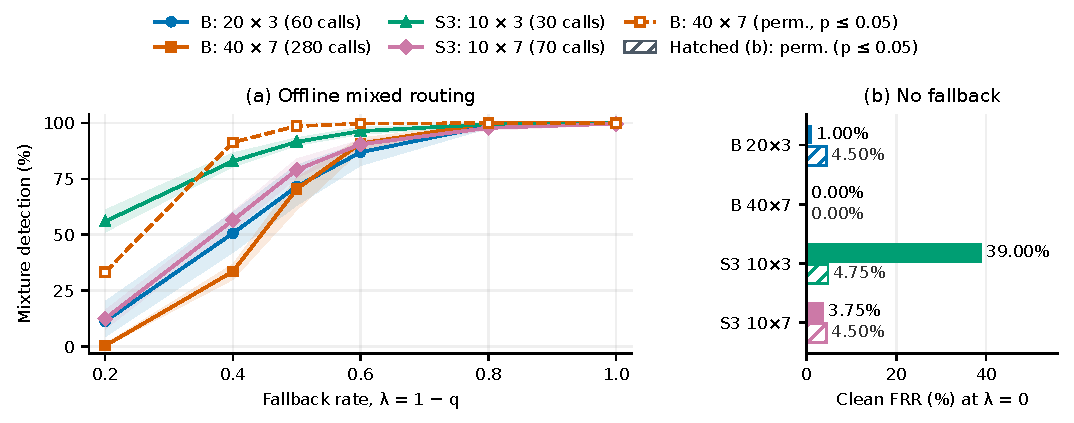
\includegraphics[width=\textwidth]{fig6_mixed_routing.pdf}
\caption{Offline mixed routing across 20 fixed seeds. Left: rejection of declared/substitute mixtures across subsampled 3- and 7-draw curves under frozen energy thresholds $\tau_{\mathrm{mid}}$ (solid, 5--95 percent seed bands) and 999-permutation testing on B $40\times 7$ ($p\le0.05$, dashed). Right: pure declared-model false rejection at $q=1$ (full-pool S3 $10\times 15$ has 0.00\% clean FRR).}\label{fig:6}
\end{figure*}

\subsection{Operational Overhead}
Table~9 separates public-rate estimated API cost, latency-replayed estimated concurrent wall time, and measured local CPU scoring excluding one-time enrollment (Supplement~K). Under November~13, 2026 OpenRouter catalog rates~\cite{ref29} (L: $0.71/0.71$ USD; G: $2.50/10.00$ USD per million input/output tokens), median 150-call S3 color query cost is 0.0077 USD (L) to 0.0345 USD (G). Scenario G spans 0.0292--0.0432 USD across 19/20 endpoints (0.2711 USD on \texttt{s3-deepseek-v3.2}; Section~4.2), and 60-call B/E audits cost under 0.02 USD. Ideal eight-worker replay of recorded single-call latencies estimates 49--116~s of network wall time across 60--150 calls. On local CPU (NumPy~2.5.5, three preloaded B fixtures; I/O, parsing, and gallery search excluded), warm single-pair medians are 0.12, 0.31, and 0.08~ms for $\Dereg{}$, and 2.39, 10.15, and 2.51~ms for 999-permutation stratified energy tests on 20-cell 3v3, 40-cell 8v7, and 10-cell 8v7 batches. Unlike eight-query multi-token classifiers~\cite{ref16} with lower round-trip latency, HuePrint runs asynchronously out-of-band to supply continuous reference margins and permutation $p$-values.

\begin{table}[t]
\centering
\caption{Median Per-Endpoint Query Overhead; Enrollment Excluded}
\label{tab:source-9}
\footnotesize
\setlength{\tabcolsep}{3pt}
\renewcommand{\arraystretch}{1.08}
\begin{tabular}{@{}>{\raggedright\arraybackslash}p{\dimexpr .17\columnwidth-6pt\relax}>{\raggedright\arraybackslash}p{\dimexpr .10\columnwidth-6pt\relax}>{\raggedright\arraybackslash}p{\dimexpr .22\columnwidth-6pt\relax}>{\raggedright\arraybackslash}p{\dimexpr .23\columnwidth-6pt\relax}>{\raggedright\arraybackslash}p{\dimexpr .14\columnwidth-6pt\relax}>{\raggedright\arraybackslash}p{\dimexpr .14\columnwidth-6pt\relax}@{}}
\toprule
Query workload & Calls & Input /\allowbreak{} output tokens & USD scenarios L /\allowbreak{} G & Call p50 (s) & Est. c=8 (s) \\
\midrule
B20x6 & 60 & 4,798.5 /\allowbreak{} 560.0 & 0.0042 /\allowbreak{} 0.0188 & 8.12 & 61.14 \\
E20x6 & 60 & 4,126.5 /\allowbreak{} 450.0 & 0.0034 /\allowbreak{} 0.0164 & 6.03 & 48.91 \\
S1\_CF21 & 120 & 9,222.0 /\allowbreak{} 980.0 & 0.0085 /\allowbreak{} 0.0357 & 3.35 & 59.49 \\
S1\_OR21 & 120 & 8,848.5 /\allowbreak{} 1,016.0 & 0.0076 /\allowbreak{} 0.0367 & 4.07 & 68.60 \\
S3\_color & 150 & 9,840.0 /\allowbreak{} 1,091.5 & 0.0077 /\allowbreak{} 0.0345 & 4.96 & 116.25 \\
S3\_word & 150 & 7,051.5 /\allowbreak{} 381.5 & 0.0054 /\allowbreak{} 0.0218 & 4.57 & 104.39 \\
S4a & 80 & 5,502.5 /\allowbreak{} 1,860.5 & 0.0051 /\allowbreak{} 0.0319 & 4.56 & 56.35 \\
\bottomrule
\end{tabular}
\par\vspace{3pt}\begin{minipage}{\columnwidth}\footnotesize Token and USD columns report medians computed independently across endpoints; substituting median input/output tokens directly into linear rate formulas therefore need not equal median USD cost.\end{minipage}
\end{table}

\section{Limitations, Deployment, and Conclusion}

\subsection{Limitations}
Ground truth relies on provider-declared labels and API logs rather than cryptographic weight attestation, so endpoint behavior alone cannot verify authorization. Shallow 3v3 cells under-sample tails, and S1's four disjoint E identities call for larger multi-month cohorts. In S2, hosts and quantization co-vary across providers, which precludes causal isolation of quantization. Under complexity cascades~\cite{ref1,ref2}, short standalone probes hit low-complexity branches, and session-level burst detectors can flag repeated probes. Both motivate workload-embedded color fields with private prompt rotation.

\subsection{Deployment Guidelines}
Consumers should bind the checkpoint, private prompts, parser, valid-count rule, and budget in a versioned audit contract:
\begin{enumerate}
    \item \textbf{Metric and estimator:} For standard monitoring, use centered $\Dereg{}$, or zero-bootstrap U-statistic ratios when $n, m \ge 2$ calibrated at matched cell budgets (signed vs.\ clipped trade off ranking and jitter FRR on E; Table~7). Across heterogeneous backends, use $\Dhyb{}$.
    \item \textbf{Calibration and two-stage verification:} Freeze $\tau_{\mathrm{mid}}$ or $\tau_{\mathrm{self}}$ where gateway drift is allowed, and apply Sz\'ekely--Rizzo permutation tests against same-gateway references for low-$\lambda$ screening. To avoid alert fatigue (where a 10\% 3v3 FRR compounds across hourly checks), verify any 3v3 crossing via an immediate 6v6 or 15v15 window before escalating.
    \item \textbf{Caching, wrapper parity, and refresh:} Screen cache hits (zero entropy at $T=1.0$ and $<0.5\times$ median latency), enroll via the identical system-prompt wrapper, corroborate alerts with task telemetry, and rotate private prompts ($<10{,}000$ tokens/model per 64-call battery) upon refresh.
\end{enumerate}

\subsection{Conclusion}
HuePrint provides a black-box behavioral consistency signal for brokered cloud LLM services below four cents median query cost. Across 34,528 cloud responses, structured RGB elicitation cuts 30-call/side EER from 4.52\%--5.23\% for the word battery to 0.94\%--1.00\% on B/D, and from 6.25\%--8.04\% to 3.49\%--5.00\% across 20 locked endpoints (0.00\% by 60--150 calls/side). Continuous and hybrid RGB distances improve shallow-census and cross-provider separation, tolerate three-week drift, and bound coordinate shifts. Together with unified Lipschitz bounds, zero-bootstrap U ratios, within-family and mixed-routing benchmarks, and structured canaries, these results support practical MaaS consistency monitoring.

\section*{Acknowledgments}
The author deeply thanks his parents and sister for their unwavering emotional and daily-life support throughout this research, and sincerely thanks his advisor, Dr.\ Vicky Li at Yunnan University of Chinese Medicine, for introducing him to computer science research.
